\begin{frame}{Aufgabe 8}
\begin{table}[]
\begin{tabular}{
>{\columncolor{gray0}}l ll}
Kenngröße                          & \cellcolor{gray0}Wert ohne Entzerrer    & \cellcolor{gray0}Wert mit Entzerrer       \\ \hline
$U_\mathrm{A}$                     & $0.4442 \, \si{\volt}$                         & \cellcolor{orange2}$0.9581 \, \si{\volt}$   \\
$U_\mathrm{R}^2$                   & $0.09136 \, \si{\volt}^2$                      & \cellcolor{orange2}$0.1452 \, \si{\volt}^2$ \\
$\rho$                             & $2.1597$                                       & $6.3220$                                         \\
$\mathrm{BER}, \mathrm{berechnet}$ & \cellcolor{red2}$7.08 \cdot 10^{-2}$   & $6.0 \cdot 10^{-3}$                              \\
$\mathrm{BER}, \mathrm{gemessen}$  & \cellcolor{red2}$3.9887 \cdot 10^{-2}$ & $7.3382 \cdot 10^{-3}$                          
\end{tabular}
\end{table}
\end{frame}

\begin{frame}{Aufgabe 8: Nyquistvektor}

  Veränderung  der Position der 1 im Nyquistvektor
  \smallgrskip

  Qualitätskriterium:
  \to Summe der quadratischen Abweichungen der Faltung {\color{cyan5}{$h(k) * f(k)$}} zu dem Nyquistvektor {\color{cyan5}{$z(k)$}}

  \smallgrskip
  \[ \sum(h(k) * f(k) - z(k) ) ^2 \rightarrow min\]

\end{frame}

\begin{frame}{Aufgabe 8: Augendiagramme}

  \twocolumns{
  \begin{center}
  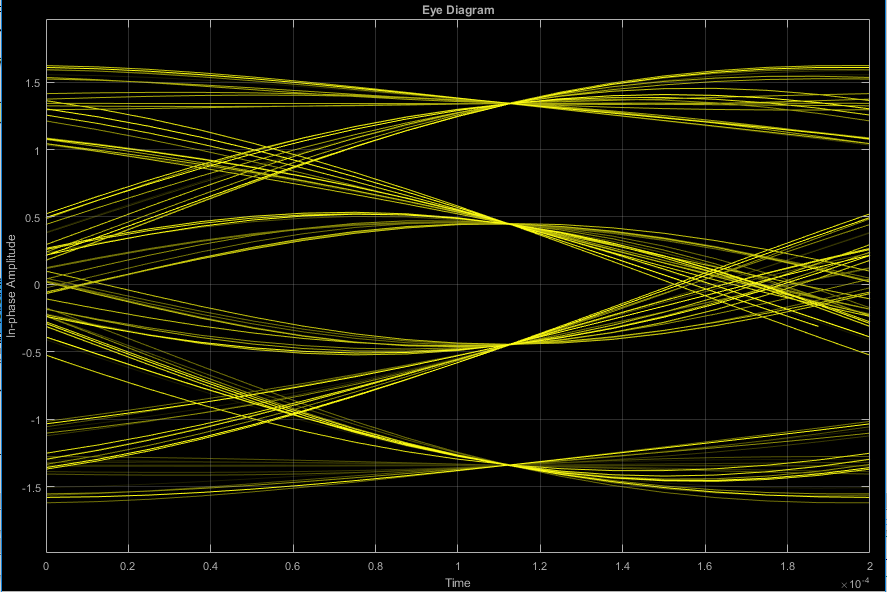
\includegraphics[width=\textwidth]{screenshots/Aufgabe8/Auge_ohne_entzerrer}
  \end{center}
} {
  \begin{center}
  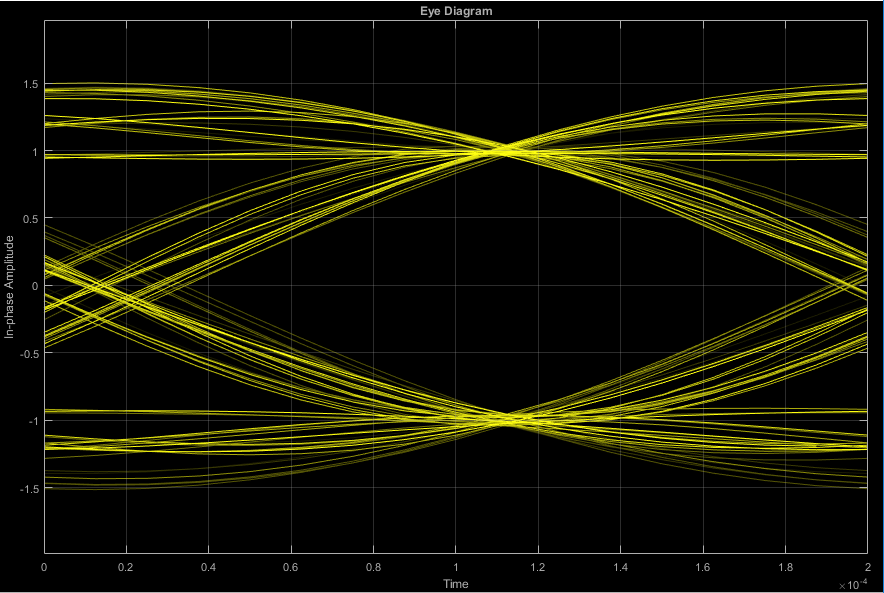
\includegraphics[width=\textwidth]{screenshots/Aufgabe8/Auge_mit_entzerrer}
  \end{center}
  
}{0.5\textwidth}
\end{frame}

\begin{frame}{Aufgabe 8: Rauschleistungsanhebung}
  \[\sum{f_i^2} = 1.654\]
\end{frame}

\begin{frame}{Aufgabe 8: BER-Vergleich}

  \twocolumns{
 Einstellung
    von $N_0$ im \textsc{SIMULINK}-Modell 
    \smallgrskip

    \[ \mathrm{SNR}_\mathrm{dB} = 10 \cdot \log_{10}{\frac{E_\mathrm{s}}{N_0}}\]

    \[N_0 = \frac{E_\mathrm{s}}{10^{\frac{\mathrm{SNR}}{10}}}\]

  }{

  \begin{center}
  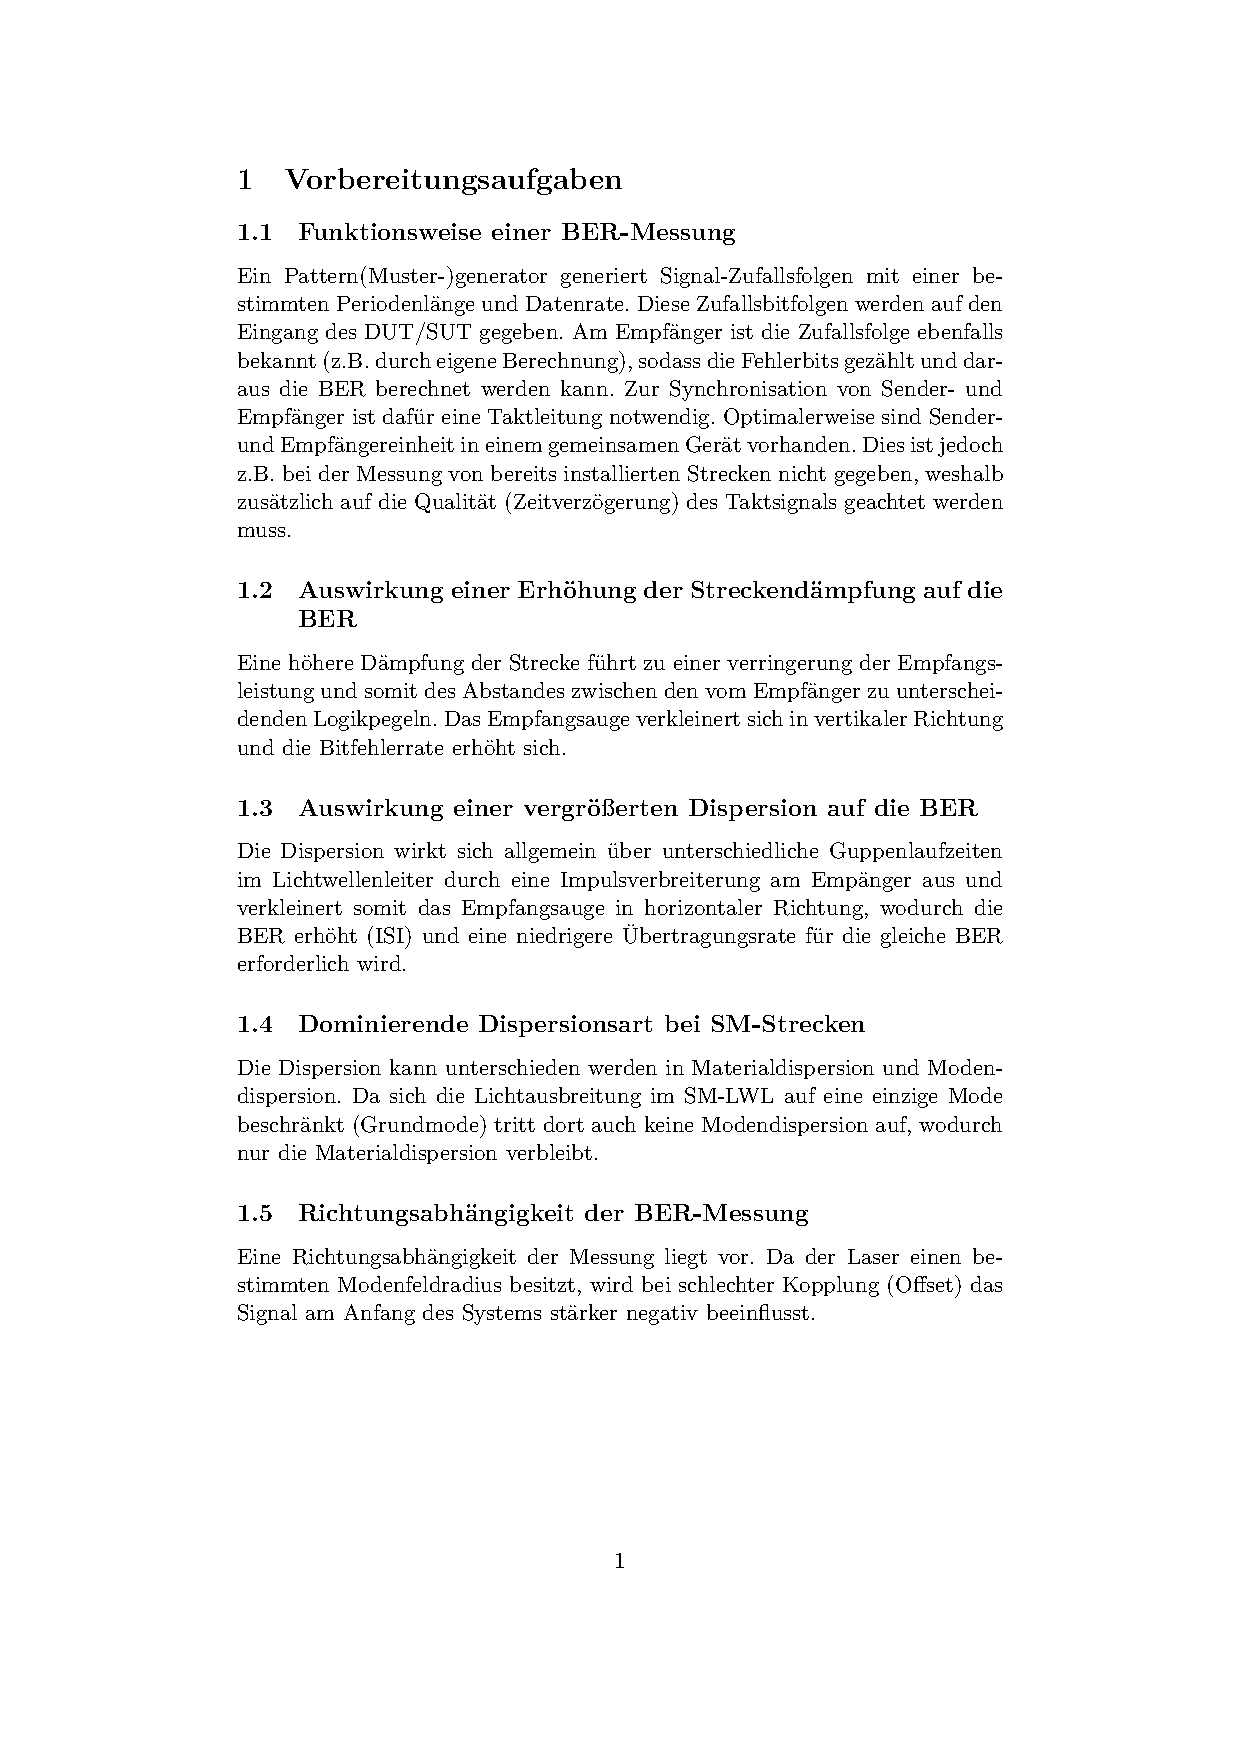
\includegraphics[width=\textwidth]{screenshots/Aufgabe8/BER}
  \end{center}

  }{0.382\textwidth}
  
\end{frame}

